\documentclass[11pt]{amsart}

\usepackage[margin=1.15in]{geometry}
\usepackage{amsmath,amssymb,amsthm}
\usepackage{enumitem}
\usepackage{tikz}
\usepackage[colorlinks=true,linkcolor=blue!60!black,citecolor=green!40!black,urlcolor=blue!60!black]{hyperref}

\newtheorem{theorem}{Theorem}[section]
\newtheorem{lemma}[theorem]{Lemma}
\newtheorem{proposition}[theorem]{Proposition}
\newtheorem{corollary}[theorem]{Corollary}
\theoremstyle{definition}
\newtheorem{definition}[theorem]{Definition}
\newtheorem{example}[theorem]{Example}
\theoremstyle{remark}
\newtheorem{remark}[theorem]{Remark}

\numberwithin{equation}{section}

\newcommand{\Zge}{\mathbb{Z}_{\ge 0}}
\newcommand{\ZZ}{\mathbb{Z}}
\newcommand{\RR}{\mathbb{R}}
\newcommand{\supp}{\operatorname{supp}}
\newcommand{\Dr}{\mathcal{D}}
\newcommand{\down}{{\downarrow}}

\title{Gamma-positivity of $h$-polynomials of preorders}

\author{Knowledge Sense}
\address{Knowledge Sense}
\email{math@knowledgesense.jp}

\date{October 7, 2026}

\subjclass[2020]{05A15, 52B20, 06A07}
\keywords{Preorder, preorder polytope, lattice point, $\gamma$-positivity, draconian sequence, perfect matching}

\begin{document}

\begin{abstract}
For a preorder $\tau$ on an $n$-element set, Athanasiadis and Chapoton defined the $h$-polynomial $h(\tau,t)$, which counts the lattice points of the preorder polytope $Q_\tau$ by their number of nonzero coordinates, and conjectured that it is $\gamma$-positive. We prove this conjecture for every finite preorder. More precisely, we show that
\[
h(\tau,t)=\sum_{j=0}^{\lfloor n/2\rfloor} b_j(\tau)\,t^j(1+t)^{n-2j},
\]
where $b_j(\tau)$ is the number of ordered pairs $(I,J)$ of disjoint $j$-element subsets for which there is a bijection $f\colon I\to J$ with $i\le f(i)$ for all $i$. The proof combines a support duality for draconian sequences of bipartite graphs, due to Dai, Hou, Liu, Thawinrak and Wang, with a short argument that reduces arbitrary pairs of subsets admitting such a bijection to disjoint ones. As special cases we recover the known $\gamma$-expansions for total orders, ordinal sums of two antichains, octopuses and lopsided octopuses.
\end{abstract}

\maketitle

\section{Introduction}\label{sec:intro}

Let $E$ be a finite set with $n$ elements. A \emph{preorder} on $E$ is a reflexive and transitive relation $\le$ on $E$. Antisymmetry is not assumed, so $\le$ may be viewed as a partial order on the blocks of a partition of $E$. A subset $U\subseteq E$ is an \emph{order ideal} if $y\in U$ and $x\le y$ imply $x\in U$. Following Athanasiadis and Chapoton~\cite{AC}, the \emph{preorder polytope} of $\tau=(E,\le)$ is
\[
Q_\tau=\Bigl\{x\in\RR_{\ge 0}^E \;:\; \sum_{e\in U}x_e\le |U| \text{ for every order ideal } U \text{ of } \tau\Bigr\},
\]
and the \emph{$h$-polynomial} of $\tau$ is
\[
h(\tau,t)=\sum_{x\in Q_\tau\cap\ZZ^E} t^{|\supp(x)|},\qquad \supp(x)=\{e\in E: x_e\neq 0\}.
\]
When $\tau$ comes from an arbor, $Q_\tau$ is the arbor polytope of Chapoton~\cite{Cha}, and $h(\tau,t)$ is the polynomial introduced there. Note that $h(\tau,t)$ is not the $h^*$-polynomial of $Q_\tau$.

A polynomial $h(t)$ is \emph{$\gamma$-positive with center of symmetry $n/2$} if $h(t)=\sum_{j=0}^{\lfloor n/2\rfloor}\gamma_j t^j(1+t)^{n-2j}$ with $\gamma_j\ge 0$. Since the polynomials $t^j(1+t)^{n-2j}$ are linearly independent, the coefficients $\gamma_j$ are uniquely determined. The $\gamma$-positivity of $h(t)$ implies that its coefficient sequence is palindromic and unimodal; see the survey~\cite{Ath18}. Athanasiadis and Chapoton~\cite[Conjecture~5.2]{AC} conjectured that $h(\tau,t)$ is $\gamma$-positive for every preorder $\tau$; for arbors this was implicit in~\cite{Cha}. They verified the conjecture by computer for all preorders of size at most~$7$. Special cases were settled earlier: chain preorders with blocks of arbitrary sizes in~\cite{Ath25}, ordinal sums of two antichains and zig-zag posets in~\cite[Section~9]{AC} (the latter using~\cite{WZC}), the arbors called octopuses in~\cite{AXY} (with a bijective proof in~\cite{Men}), and lopsided octopuses in~\cite{Men}.

In this paper we prove the conjecture in general, with an explicit combinatorial description of the $\gamma$-coefficients.

\begin{definition}\label{def:upward}
Let $I,J\subseteq E$. An \emph{upward bijection} from $I$ to $J$ is a bijection $f\colon I\to J$ such that $i\le f(i)$ for every $i\in I$. For $0\le j\le \lfloor n/2\rfloor$, let $b_j(\tau)$ be the number of ordered pairs $(I,J)$ of \emph{disjoint} $j$-element subsets of $E$ for which an upward bijection $I\to J$ exists.
\end{definition}

Here $i$ and $f(i)$ may lie in the same block of $\tau$. Each pair $(I,J)$ is counted once, even if several upward bijections $I\to J$ exist. The empty pair gives $b_0(\tau)=1$.

\begin{theorem}\label{thm:main}
For every preorder $\tau$ on an $n$-element set,
\begin{equation}\label{eq:main}
h(\tau,t)=\sum_{j=0}^{\lfloor n/2\rfloor} b_j(\tau)\, t^j(1+t)^{n-2j}.
\end{equation}
In particular, $h(\tau,t)$ is $\gamma$-positive with $\gamma_j(\tau)=b_j(\tau)$, and Conjecture~5.2 of~\cite{AC} holds.
\end{theorem}

Theorem~\ref{thm:main} implies Conjecture~5.1(b) of~\cite{AC}, the palindromicity and unimodality of $h(\tau,t)$ for every preorder $\tau$. Since arbors are special preorders, it gives in particular the palindromicity and unimodality of $h(\sigma,t)$ for every arbor $\sigma$, which Chapoton~\cite{Cha} conjectured as part of a stronger statement.

\begin{corollary}\label{cor:consequences}
Let $\tau$ be a preorder of size $n$ and let $\tau^*$ be its dual preorder.
\begin{enumerate}[label=\textup{(\alph*)}]
\item The coefficient sequence of $h(\tau,t)$ is palindromic and unimodal.
\item $b_j(\tau)=b_j(\tau^*)$ for all $j$; hence $h(\tau,t)=h(\tau^*,t)$.
\item $b_1(\tau)$ is the number of ordered pairs $(x,y)$ of elements of $E$ with $x\ne y$ and $x\le y$.
\end{enumerate}
\end{corollary}

\begin{proof}
Part (a) is a standard consequence of $\gamma$-positivity. For (b), if $f\colon I\to J$ is an upward bijection for $\tau$, then $f^{-1}\colon J\to I$ is an upward bijection for $\tau^*$, so $(I,J)\mapsto(J,I)$ is a bijection between the pairs counted by $b_j(\tau)$ and by $b_j(\tau^*)$. Part (c) is the case $j=1$ of Definition~\ref{def:upward}.
\end{proof}

The identity $h(\tau,t)=h(\tau^*,t)$ is Conjecture~5.4 of~\cite{AC}, proved by Dai, Hou, Liu, Thawinrak and Wang~\cite{DHLTW}. Since our argument uses their duality theorem, Corollary~\ref{cor:consequences}(b) is not an independent proof.

\subsection*{Relation to previous work}
Apart from Hall's theorem, the only result we use is the support duality of Dai, Hou, Liu, Thawinrak and Wang~\cite[Theorem~1.3]{DHLTW}, recalled as Theorem~\ref{thm:DHLTW}. From it we derive Lemma~\ref{lem:fullsupport}, which states that the number of draconian sequences with full support equals the number of vertex subsets admitting a perfect matching. Statements of this type are known; for instance, Ohsugi and Tsuchiya~\cite[Proposition~3.4]{OT} describe interior polynomials in terms of vertex sets of matchings (see Remark~\ref{rem:OT}). The new ingredient is the passage from all pairs $(I,J)$ admitting an upward bijection to disjoint ones (Lemma~\ref{lem:cancel}), which yields the expansion~\eqref{eq:main}.

The paper is organized as follows. Section~\ref{sec:prelim} recalls the duality theorem and derives the counting lemma. Section~\ref{sec:proof} proves Theorem~\ref{thm:main}, and Section~\ref{sec:second} gives a second derivation. Section~\ref{sec:examples} treats examples, Section~\ref{sec:computation} reports a computational check, and Section~\ref{sec:remarks} contains concluding remarks.

\section{Draconian sequences and a counting lemma}\label{sec:prelim}

Let $H$ be a finite bipartite graph with vertex classes $L$ and $R$. For $A\subseteq L$ write $N_H(A)\subseteq R$ for the set of neighbors of $A$. Following~\cite[Definition~1.1]{DHLTW}, which is a variant of Postnikov's notion~\cite{Pos}, let
\[
\Dr(H)=\Bigl\{a\in\Zge^{L} \;:\; \sum_{i\in A}a_i\le |N_H(A)| \text{ for every } A\subseteq L\Bigr\}
\]
be the set of \emph{$H$-draconian sequences}, and let $F_H(s)=\sum_{a\in\Dr(H)} s^{|\supp(a)|}$ be its support enumerator. In contrast with Postnikov's original definition, the total sum $\sum_i a_i$ is not required to take a fixed value; it is only bounded above by $|N_H(L)|$. Let $H^*$ denote the same graph with the roles of $L$ and $R$ interchanged.

\begin{theorem}[{\cite[Theorem~1.3]{DHLTW}}]\label{thm:DHLTW}
For every finite bipartite graph $H$, one has $F_H(s)=F_{H^*}(s)$.
\end{theorem}

The graphs to which we apply Theorem~\ref{thm:DHLTW} may have isolated vertices or an empty vertex class. These cases reduce directly to graphs with neither. Indeed, if $v$ is an isolated vertex of $H$ in $L$, then every $a\in\Dr(H)$ satisfies $a_v\le|N_H(\{v\})|=0$, while in $H^*$ the vertex $v$ lies in no neighborhood; so deleting $v$ changes neither $F_H$ nor $F_{H^*}$. The same holds for an isolated vertex in $R$, by symmetry. After all isolated vertices are deleted, either both classes are nonempty, or the graph has no vertices, in which case $F_H=F_{H^*}=1$.

\begin{lemma}\label{lem:fullsupport}
Let $H$ be a bipartite graph with vertex classes $L$ and $R$, and let $k=|L|$. Then
\[
\#\{a\in\Dr(H) : \supp(a)=L\}=\#\{I\subseteq R : |I|=k \text{ and } H[L\sqcup I] \text{ has a perfect matching}\}.
\]
\end{lemma}

\begin{proof}
The left-hand side is the coefficient of $s^k$ in $F_H(s)$, because every $a\in\Dr(H)$ has support contained in $L$. By Theorem~\ref{thm:DHLTW} it equals the number of $b\in\Dr(H^*)$ with exactly $k$ positive entries. Taking $A=R$ in the definition of $\Dr(H^*)$ gives $\sum_{r\in R}b_r\le|N_{H^*}(R)|\le k$, so such a vector $b$ is the indicator vector $\mathbf 1_I$ of a $k$-element subset $I\subseteq R$. It remains to decide when $\mathbf 1_I\in\Dr(H^*)$. If $|B|\le|N_{H^*}(B)|$ for every $B\subseteq I$, then for every $A\subseteq R$ we have $|A\cap I|\le|N_{H^*}(A\cap I)|\le|N_{H^*}(A)|$. Hence $\mathbf 1_I\in\Dr(H^*)$ if and only if $|B|\le|N_{H^*}(B)|$ for all $B\subseteq I$, and since $|I|=|L|$, by Hall's theorem~\cite{Hall} this holds if and only if $H[L\sqcup I]$ has a perfect matching.
\end{proof}

\section{Proof of Theorem~\ref{thm:main}}\label{sec:proof}

Fix a preorder $\tau=(E,\le)$. For $Y\subseteq E$ let $\down Y=\{e\in E: e\le y \text{ for some } y\in Y\}$. By reflexivity and transitivity, $\down Y$ is the smallest order ideal containing $Y$.

For $J\subseteq E$, let $H_J$ be the bipartite graph with vertex classes $J$ and a disjoint copy of $E$, in which $j\in J$ is adjacent to $i\in E$ if and only if $i\le j$. Thus $N_{H_J}(Y)=\down Y$ for every $Y\subseteq J$.

\begin{lemma}\label{lem:reduction}
Let $J\subseteq E$ and let $x\in\Zge^E$ with $\supp(x)=J$. Then $x\in Q_\tau$ if and only if the restriction $x|_J$ belongs to $\Dr(H_J)$.
\end{lemma}

\begin{proof}
Suppose $x\in Q_\tau$ and let $Y\subseteq J$. Since $x$ is nonnegative and vanishes off $J$, and $\down Y$ is an order ideal containing $Y$,
\[
\sum_{j\in Y}x_j\le \sum_{e\in\down Y}x_e\le|\down Y|=|N_{H_J}(Y)|.
\]
Conversely, suppose $x|_J\in\Dr(H_J)$ and let $U$ be an order ideal. Put $Y=J\cap U$. Then $N_{H_J}(Y)=\down Y\subseteq U$, hence $\sum_{e\in U}x_e=\sum_{j\in Y}x_j\le|N_{H_J}(Y)|\le|U|$.
\end{proof}

By Lemma~\ref{lem:reduction}, the number of lattice points of $Q_\tau$ with support exactly $J$ equals the number of elements of $\Dr(H_J)$ with full support $J$. By Lemma~\ref{lem:fullsupport}, this is the number of subsets $I\subseteq E$ with $|I|=|J|$ for which $H_J[J\sqcup I]$ has a perfect matching. A perfect matching of $H_J[J\sqcup I]$ is the same as an upward bijection $I\to J$. Summing over $J$ we obtain
\begin{equation}\label{eq:overlap}
h(\tau,t)=\sum_{(I,J)} t^{|J|},
\end{equation}
where the sum runs over all ordered pairs $(I,J)$ of subsets of $E$, \emph{not necessarily disjoint}, for which an upward bijection $I\to J$ exists. Each such pair is counted once.

It remains to remove the elements common to $I$ and $J$. For a pair $(I,J)$ put
\[
A=I\setminus J,\qquad B=J\setminus I,\qquad K=I\cap J .
\]

\begin{lemma}\label{lem:cancel}
There is an upward bijection $I\to J$ if and only if there is an upward bijection $A\to B$.
\end{lemma}

\begin{proof}
Suppose $f\colon I\to J$ is an upward bijection, and consider the directed graph on $I\cup J$ with arrows $i\to f(i)$. Each vertex of $A$ has out-degree $1$ and in-degree $0$, each vertex of $B$ has in-degree $1$ and out-degree $0$, and each vertex of $K$ has in-degree and out-degree $1$. Hence the connected components are directed cycles contained in $K$ (including loops $f(i)=i$) and directed paths that start in $A$, pass through $K$ and end in $B$. Every element of $A$ starts exactly one path and every element of $B$ ends exactly one path. Sending the initial vertex of each path to its terminal vertex defines a bijection $g\colon A\to B$, and transitivity applied along each path gives $a\le g(a)$.

Conversely, if $g\colon A\to B$ is an upward bijection, then $g$ together with the identity map of $K$ is an upward bijection $I\to J$, by reflexivity.
\end{proof}

\begin{proof}[Proof of Theorem~\ref{thm:main}]
The map $(I,J)\mapsto (A,B,K)$ is a bijection from ordered pairs of subsets of $E$ with $|I|=|J|$ to triples of pairwise disjoint subsets with $|A|=|B|$; its inverse is $(A,B,K)\mapsto(A\cup K,B\cup K)$, and $|J|=|B|+|K|$. By Lemma~\ref{lem:cancel}, the pairs occurring in~\eqref{eq:overlap} correspond to the triples in which $(A,B)$ is one of the disjoint pairs counted by $b_j(\tau)$, where $j=|A|\le\lfloor n/2\rfloor$, and $K$ is an arbitrary subset of the $(n-2j)$-element set $E\setminus(A\cup B)$. Therefore
\[
h(\tau,t)=\sum_{j=0}^{\lfloor n/2\rfloor}\ \sum_{(A,B)} \ \sum_{K\subseteq E\setminus(A\cup B)} t^{\,j+|K|}
=\sum_{j=0}^{\lfloor n/2\rfloor} b_j(\tau)\,t^j(1+t)^{n-2j},
\]
where $(A,B)$ runs over the pairs counted by $b_j(\tau)$.
\end{proof}

\begin{remark}\label{rem:axioms}
The preorder axioms enter the proof in three places: reflexivity and transitivity make $\down Y$ the smallest order ideal containing $Y$ (Lemma~\ref{lem:reduction}), transitivity shortens paths in Lemma~\ref{lem:cancel}, and reflexivity extends a bijection $A\to B$ by the identity on $K$.
\end{remark}

\section{A second derivation}\label{sec:second}

We sketch an equivalent derivation, which produces the disjoint pairs directly. For $x\in\Zge^E$ put
\[
Z=\{e: x_e=0\},\qquad J=\{e : x_e\ge 2\},\qquad d_a=x_a-1\ \ (a\in J),
\]
so that $d_a$ is the excess of $x_a$ over $1$. For every $U\subseteq E$ one has $\sum_{e\in U}x_e-|U|=\sum_{a\in J\cap U}d_a-|Z\cap U|$. Let $H_{J,Z}$ be the bipartite graph with vertex classes $J$ and $Z$, in which $a\in J$ is adjacent to $z\in Z$ when $z\le a$. Arguing as in Lemma~\ref{lem:reduction} (apply the defining inequality to $\down Y$ for $Y\subseteq J$, and for an order ideal $U$ use $Y=J\cap U$ and $N_{H_{J,Z}}(Y)\subseteq Z\cap U$), one finds that $x\in Q_\tau$ if and only if $d\in\Dr(H_{J,Z})$; note that $d$ has full support $J$. By Lemma~\ref{lem:fullsupport}, for fixed disjoint $Z$ and $J$ the number of such $x$ equals the number of $j$-element subsets $I\subseteq Z$, $j=|J|$, admitting an upward bijection $I\to J$. Since $|\supp(x)|=n-|Z|$, reordering the finite sum gives
\[
h(\tau,t)=\sum_{(I,J)}\ \sum_{I\subseteq Z\subseteq E\setminus J} t^{\,n-|Z|}=\sum_{j=0}^{\lfloor n/2\rfloor}b_j(\tau)\,t^j(1+t)^{n-2j},
\]
where $(I,J)$ runs over the disjoint pairs counted by the numbers $b_j(\tau)$. Here the coordinates equal to $1$ play the role of the set $K$ in Section~\ref{sec:proof}.

\section{Examples}\label{sec:examples}

In each of the following cases $b_j(\tau)$ is computed directly from Definition~\ref{def:upward}.

\begin{example}[Antichains and a single block]
If $\tau$ is an antichain, the only upward bijections are identity maps, so $b_j(\tau)=0$ for $j\ge 1$ and $h(\tau,t)=(1+t)^n$. If $\tau$ has a single block of size $n$, every pair of disjoint subsets of equal size qualifies, and $b_j(\tau)=\binom{n}{j}\binom{n-j}{j}$.
\end{example}

\begin{example}[Total orders]
Let $\tau$ be the total order $1<2<\dots<n$, that is, the chain preorder all of whose blocks are singletons. For disjoint $I=\{u_1<\dots<u_j\}$ and $J=\{v_1<\dots<v_j\}$, an upward bijection exists if and only if $u_k<v_k$ for all $k$. Choosing the $2j$ elements of $I\cup J$ and then a ballot sequence gives
\[
b_j(\tau)=\binom{n}{2j}C_j,\qquad C_j=\frac{1}{j+1}\binom{2j}{j}.
\]
This is the classical $\gamma$-expansion of the Narayana polynomial (see~\cite{Ath18}), in agreement with~\cite{Cha}, where $h(\tau,t)$ is identified with the $h$-polynomial of the associahedron of type $A_n$. Chain preorders with larger blocks are covered by Theorem~\ref{thm:main} and by~\cite{Ath25}; we do not compute their coefficients here.
\end{example}

\begin{example}[Ordinal sum of two antichains]
Let $\tau$ be the ordinal sum of an antichain of size $p$ below an antichain of size $q$. An element of the top level lies below no element other than itself, and distinct elements of the bottom level are incomparable. Hence a disjoint pair $(I,J)$ admits an upward bijection exactly when $I$ lies in the bottom level and $J$ in the top level, and $b_j(\tau)=\binom{p}{j}\binom{q}{j}$. This recovers~\cite[Proposition~9.2]{AC}.
\end{example}

\begin{example}[Octopuses and lopsided octopuses]
Let $n,k_1,k_2\ge 0$ with $k=k_1+2k_2<n$, and let $\tau$ be the lopsided octopus of~\cite{Men}: a root block $R$ of size $n-k$, together with $k_1$ singleton leaves and $k_2$ two-element leaves, each leaf lying directly below $R$. An element of $R$ lies below only elements of $R$, and an element of a leaf lies below only $R$ and the elements of its own leaf. Consider a disjoint pair $(I,J)$ with an upward bijection. No element of $J$ lies in a singleton leaf, and an element of $J$ lying in a two-element leaf must be matched with the other element of that leaf; all other elements of $J$ lie in $R$, and they can be matched with arbitrary remaining elements. If exactly $i$ two-element leaves meet $J$, there are $2^i\binom{k_2}{i}$ choices for these leaves and for the element of each of them lying in $J$, then $\binom{n-k}{j-i}$ choices for $J\cap R$, and $\binom{n-j-i}{j-i}$ choices for the remaining $j-i$ elements of $I$, which are taken outside $J$ and outside the $i$ chosen leaves. Thus
\[
b_j(\tau)=\sum_{i=0}^{k_2}2^i\binom{k_2}{i}\binom{n-k}{j-i}\binom{n-j-i}{j-i},
\]
which is~\cite[Proposition~3.4]{Men}. For $k_2=0$ this is $\binom{n-k}{j}\binom{n-j}{j}$, the formula of Athanasiadis, Xiao and Yan~\cite[Proposition~2.2]{AXY} for octopuses.
\end{example}

\begin{example}[A poset that is not an arbor]\label{ex:eight}
Let $E=\{a_1,a_2,a_3,d,c_0,c_1,c_2,c_3\}$ with the strict relations $a_i<c_0$, $a_i<c_i$ and $d<c_i$ for $i=1,2,3$; see Figure~\ref{fig:eight}. Then
\[
h(\tau,t)=1+17t+106t^2+303t^3+427t^4+303t^5+106t^6+17t^7+t^8,
\]
so that $(b_0(\tau),\dots,b_4(\tau))=(1,9,24,16,1)$. Here $b_1(\tau)=9$ is the number of ordered pairs $x\ne y$ with $x\le y$, which are the strict relations since $\tau$ is a poset; this is in agreement with Corollary~\ref{cor:consequences}(c). Also $b_4(\tau)=1$, because $(\{a_1,a_2,a_3,d\},\{c_0,c_1,c_2,c_3\})$ is the only disjoint pair of $4$-element sets with an upward bijection.
\end{example}

\begin{figure}[ht]
\centering
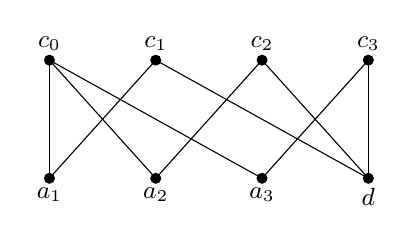
\begin{tikzpicture}[x=1.35cm,y=1.5cm,every node/.style={font=\small}]
\foreach \name/\xx in {a1/0,a2/1,a3/2,d/3}{\coordinate (\name) at (\xx,0);}
\foreach \name/\xx in {c0/0,c1/1,c2/2,c3/3}{\coordinate (\name) at (\xx,1);}
\foreach \i in {1,2,3}{\draw (a\i)--(c0); \draw (a\i)--(c\i); \draw (d)--(c\i);}
\foreach \name/\lab in {a1/a_1,a2/a_2,a3/a_3,d/d}{\fill (\name) circle (2pt); \node[below] at (\name) {$\lab$};}
\foreach \name/\lab in {c0/c_0,c1/c_1,c2/c_2,c3/c_3}{\fill (\name) circle (2pt); \node[above] at (\name) {$\lab$};}
\end{tikzpicture}
\caption{The Hasse diagram of the poset of Example~\ref{ex:eight}.}
\label{fig:eight}
\end{figure}

\section{Computational check}\label{sec:computation}

An exact enumeration in integer arithmetic confirms~\eqref{eq:main} for all $7{,}332$ labeled preorders on at most five elements, a count that includes the empty preorder, for $100$ pseudorandom preorders on six to eight elements, and for Example~\ref{ex:eight}. It also confirms Theorem~\ref{thm:DHLTW} and Lemma~\ref{lem:fullsupport} for all $689$ labeled bipartite graphs with at most three vertices in each class. The program enumerates lattice points of $Q_\tau$ directly from the order-ideal inequalities and computes $b_j(\tau)$ by testing for the existence of an upward bijection. These computations are not part of the proof. The program is available from the author.

\section{Concluding remarks}\label{sec:remarks}

\begin{remark}[Interior polynomials]\label{rem:OT}
Let $G_\tau$ be the bipartite graph whose vertex classes are two copies of $E$, with $i$ in the first copy adjacent to $j$ in the second whenever $i\le j$. The pairs $(I,J)$ in~\eqref{eq:overlap} are exactly the pairs of vertex sets of matchings of $G_\tau$, so~\eqref{eq:overlap} is a generating function of the type that Ohsugi and Tsuchiya~\cite[Proposition~3.4]{OT} use to describe interior polynomials. In~\cite[Theorem~0.3]{OT}, numbers of such vertex sets, multiplied by powers of $4$, appear as $\gamma$-coefficients of the $h^*$-polynomial of a different reflexive polytope $\mathcal{B}_G$; that result concerns a different polynomial from $h(\tau,t)$.
\end{remark}

\begin{remark}[Scope]
Theorem~\ref{thm:main} implies Conjectures~5.1(a), 5.1(b) and 5.2 of~\cite{AC}. It does not address the realization of $h(\tau,t)$ as the $h$-polynomial of a (flag) simplicial polytope~\cite[Conjecture~5.1(c),(d)]{AC}, the real-rootedness of $h(\tau,t)$~\cite[Conjecture~5.3]{AC}, or the conjectures of~\cite{AC} on the $h^*$-polynomial of $Q_\tau$. Since $h(\tau,t)$ is $\gamma$-positive, its real-rootedness is equivalent to that of the polynomial $\sum_j b_j(\tau)t^j$.
\end{remark}

\section*{Acknowledgments}
AI-assisted tools were used in the research and preparation of this manuscript.

\begin{thebibliography}{99}

\bibitem{Ath18}
C.~A. Athanasiadis, \emph{Gamma-positivity in combinatorics and geometry}, S\'em. Lothar. Combin. \textbf{77} (2018), Article B77i.

\bibitem{Ath25}
C.~A. Athanasiadis, \emph{Lattice point enumeration of polytopes associated to integer compositions}, Ann. Comb. (2026), \href{https://doi.org/10.1007/s00026-026-00812-2}{doi:10.1007/s00026-026-00812-2}.

\bibitem{AC}
C.~A. Athanasiadis and F.~Chapoton, \emph{Polytopes and posets associated to preorders}, arXiv:2605.26916v1 (2026).

\bibitem{AXY}
C.~A. Athanasiadis, Q.~Xiao and X.~Yan, \emph{Lattice point enumeration of some arbor polytopes}, arXiv:2603.11654 (2026).

\bibitem{Cha}
F.~Chapoton, \emph{On posets and polytopes attached to arbors}, Math. Scand. \textbf{131} (2025), 401--449.

\bibitem{DHLTW}
Z.~Dai, Q.~Hou, Z.~Liu, W.~Thawinrak and H.~Wang, \emph{Counting lattice points in Minkowski sums of cross polytopes}, arXiv:2608.16037v2 (2026).

\bibitem{Hall}
P.~Hall, \emph{On representatives of subsets}, J. London Math. Soc. \textbf{10} (1935), 26--30.

\bibitem{Men}
K.~Menon, \emph{Gamma-positivity for octopuses: a bijective proof}, arXiv:2608.13247v1 (2026).

\bibitem{OT}
H.~Ohsugi and A.~Tsuchiya, \emph{Reflexive polytopes arising from bipartite graphs with $\gamma$-positivity associated to interior polynomials}, Selecta Math. (N.S.) \textbf{26} (2020), Article 59, \href{https://doi.org/10.1007/s00029-020-00588-0}{doi:10.1007/s00029-020-00588-0}.

\bibitem{Pos}
A.~Postnikov, \emph{Permutohedra, associahedra, and beyond}, Int. Math. Res. Not. IMRN \textbf{2009} (2009), 1026--1106.

\bibitem{WZC}
Y.~Wang, S.-N. Zheng and X.~Chen, \emph{Analytic aspects of Delannoy numbers}, Discrete Math. \textbf{342} (2019), 2270--2277.

\end{thebibliography}

\end{document}